\documentclass[UTF8,a4paper,10pt]{ctexart}
\usepackage[left=3.17cm, right=3.17cm, top=2.74cm, bottom=2.74cm]{geometry}
\usepackage{amsmath}
\usepackage{graphicx,subfig}
\usepackage{float}
\usepackage{cite}
\usepackage{caption}
\usepackage{enumerate}
\usepackage{booktabs} %表格
\usepackage{multirow}
\newcommand{\tabincell}[2]{\begin{tabular}{@{}#1@{}}#2\end{tabular}}  %表格强制换行
%-------------------------字体设置--------------
\usepackage{times} 
\setmainfont{TimesNewRomanPSMT}%英文一律使用times new roman
%楷体\kaishu  黑体\heiti 仿宋\fangsong 隶书\lishu  幼圆\youyuan
% \setCJKmainfont[BoldFont=Kaiti SC Bold]{Kaiti SC}   %大概是唯一一个有粗体的楷体_(:з」∠)_
\setCJKfamilyfont{kt}[BoldFont=Kaiti SC Bold]{Kaiti SC}
\newcommand{\kt}{\CJKfamily{kt}}  
\newcommand{\song}{\CJKfamily{song}}    % 宋体
\newcommand{\fs}{\CJKfamily{fs}}             % 仿宋体
\setCJKfamilyfont{hwkt}{STKaiti} %引用华文楷体
\newcommand{\hwkt}{\CJKfamily{hwkt}} 
\setCJKfamilyfont{hwxk}{STXingkai} %引用华文行楷
\newcommand{\hwxk}{\CJKfamily{hwxk}}
\newcommand{\yihao}{\fontsize{26pt}{36pt}\selectfont}           % 一号, 1.4 倍行距
\newcommand{\erhao}{\fontsize{22pt}{28pt}\selectfont}          % 二号, 1.25倍行距
\newcommand{\xiaoer}{\fontsize{18pt}{18pt}\selectfont}          % 小二, 单倍行距
\newcommand{\sanhao}{\fontsize{16pt}{24pt}\selectfont}  %三号字
\newcommand{\xiaosan}{\fontsize{15pt}{22pt}\selectfont}        % 小三, 1.5倍行距
\newcommand{\sihao}{\fontsize{14pt}{21pt}\selectfont}            % 四号, 1.5 倍行距
\newcommand{\banxiaosi}{\fontsize{13pt}{19.5pt}\selectfont}    % 半小四, 1.5倍行距
\newcommand{\xiaosi}{\fontsize{12pt}{18pt}\selectfont}            % 小四, 1.5倍行距
\newcommand{\dawuhao}{\fontsize{11pt}{11pt}\selectfont}       % 大五号, 单倍行距
\newcommand{\wuhao}{\fontsize{10.5pt}{15.75pt}\selectfont}    % 五号, 单倍行距
%-------------------------章节名----------------
\usepackage{ctexcap} 
\CTEXsetup[name={,、},number={ \chinese{section}}]{section}
\CTEXsetup[name={(,)},number={\chinese{subsection}}]{subsection}
\CTEXsetup[name={,.},number={\arabic{subsubsection}}]{subsubsection}
%-------------------------页眉页脚--------------
\usepackage{fancyhdr}
\pagestyle{fancy}
\lhead{\kaishu \leftmark}
% \chead{}
\rhead{\kaishu 系统综合课程设计实验报告}%加粗\bfseries 
\lfoot{}
\cfoot{\thepage}
\rfoot{}
\renewcommand{\headrulewidth}{0.1pt}  
\renewcommand{\footrulewidth}{0pt}%去掉横线
\newcommand{\HRule}{\rule{\linewidth}{0.5mm}}%标题横线
\newcommand{\HRulegrossa}{\rule{\linewidth}{1.2mm}}
%-----------------------伪代码------------------
\usepackage{algorithm}  
\usepackage{algorithmicx}  
\usepackage{algpseudocode}  
\floatname{algorithm}{Algorithm}  
\renewcommand{\algorithmicrequire}{\textbf{Input:}}  
\renewcommand{\algorithmicensure}{\textbf{Output:}} 
\usepackage{lipsum}  
\makeatletter
\newenvironment{breakablealgorithm}
  {% \begin{breakablealgorithm}
   \begin{center}
     \refstepcounter{algorithm}% New algorithm
     \hrule height.8pt depth0pt \kern2pt% \@fs@pre for \@fs@ruled
     \renewcommand{\caption}[2][\relax]{% Make a new \caption
       {\raggedright\textbf{\ALG@name~\thealgorithm} ##2\par}%
       \ifx\relax##1\relax % #1 is \relax
         \addcontentsline{loa}{algorithm}{\protect\numberline{\thealgorithm}##2}%
       \else % #1 is not \relax
         \addcontentsline{loa}{algorithm}{\protect\numberline{\thealgorithm}##1}%
       \fi
       \kern2pt\hrule\kern2pt
     }
  }{% \end{breakablealgorithm}
     \kern2pt\hrule\relax% \@fs@post for \@fs@ruled
   \end{center}
  }
\makeatother
%------------------------代码-------------------
\usepackage{xcolor} 
\usepackage{listings} 
\lstset{ 
breaklines,%自动换行
basicstyle=\small,
escapeinside=``,
keywordstyle=\color{ blue!70} \bfseries,
commentstyle=\color{red!50!green!50!blue!50},% 
stringstyle=\ttfamily,% 
extendedchars=false,% 
linewidth=\textwidth,% 
numbers=left,% 
numberstyle=\tiny \color{blue!50},% 
frame=trbl% 
rulesepcolor= \color{ red!20!green!20!blue!20} 
}
%------------超链接----------
\usepackage[colorlinks,linkcolor=black,anchorcolor=blue]{hyperref}
%------------------------TODO-------------------
\usepackage{enumitem,amssymb}
\newlist{todolist}{itemize}{2}
\setlist[todolist]{label=$\square$}
% for check symbol 
\usepackage{pifont}
\newcommand{\cmark}{\ding{51}}%
\newcommand{\xmark}{\ding{55}}%
\newcommand{\done}{\rlap{$\square$}{\raisebox{2pt}{\large\hspace{1pt}\cmark}}\hspace{-2.5pt}}
\newcommand{\wontfix}{\rlap{$\square$}{\large\hspace{1pt}\xmark}}
%------------------------水印-------------------
\usepackage{tikz}
\usepackage{xcolor}
\usepackage{eso-pic}

\newcommand{\watermark}[3]{\AddToShipoutPictureBG{
\parbox[b][\paperheight]{\paperwidth}{
\vfill%
\centering%
\tikz[remember picture, overlay]%
  \node [rotate = #1, scale = #2] at (current page.center)%
    {\textcolor{gray!80!cyan!30!magenta!30}{#3}};
\vfill}}}
%----------------------------------------------
\begin{document}
\begin{titlepage}
    \begin{center}
    
\includegraphics[width=0.8\textwidth]{fig/NKU.png}\\[1cm]    
    \textsc{\Huge \kaishu{\textbf{南\ \ \ \ \ \ 开\ \ \ \ \ \ 大\ \ \ \ \ \ 学}} }\\[0.9cm]
    \textsc{\huge \kaishu{\textbf{计\ \ 算\ \ 机\ \ 学\ \ 院}}}\\[0.5cm]
    \textsc{\Large \textbf{系统综合课程设计实验报告}}\\[0.8cm]
    \HRule \\[0.9cm]
    { \LARGE \bfseries PA4实验报告+PA5浮点数部分实验报告}\\[0.4cm]
    \HRule \\[2.0cm]
    \centering
    \textsc{\LARGE \kaishu{\ \ \ \ 周辰霏1712991}}\\[0.5cm]
    \textsc{\LARGE \kaishu{年级\ :\ 2017级}}\\[0.5cm]
    \textsc{\LARGE \kaishu{专业\ :\ 计算机科学与技术}}\\[0.5cm]
    \vfill
    {\Large \today}
    \end{center}
\end{titlepage}
%----------------------------------------没想好摘要写什么不写了-----------------------------------------------------------
% \newpage
% \thispagestyle{empty}
% \renewcommand{\abstractname}{\kaishu \sihao \textbf{摘要}}
%     \begin{abstract}
%         \kt{实现基于Phong模型的光线跟踪渲染器,实现全部基础功能以及任意obj文件的渲染和纹理的附加功能。 

%         在此附上\href{https://github.com/TiffanyChou21/COSC-0035-CG/tree/master/Phong}{GitHub仓库}以及\href{https://cdn.jsdelivr.net/gh/TiffanyChou21/CDN/video/Phong.mp4}{演示Demo}  }   
%         \noindent  %顶格
%         \kt{\textbf{\\\ 关键字:}\textbf{Phong模型;光线跟踪;蒙特卡罗;C++} \\\ \\\ } 
%     \end{abstract}
%---------------------------------------------------------------------------------------------------
\tableofcontents
%---------------------------------------------------------------------------------------------------
\newpage
\watermark{60}{10}{PA4\&5}
\setcounter{page}{1}
\section{概述}
%——————————————————————————————————————
\subsection{实验目的}
\kt{
    \begin{itemize}
        \item 实现内存管理单元以及虚拟内存的分页机制
        \item 实现上下文切换并可以对多任务进程进行切换
    \end{itemize}

    分时多任务实际上就是最早的UNIX批处理系统,在程序员发出指令或者OS自身可以进行任务(进程)的切换。而PA4就是在内存系统上最终实现这一系统。
}
%——————————————————————————————————————
\subsection{实验内容}
\kt{
    PA3实验涉及现代指令系统的实现、抽象机器AM 的原理与应用、输入输出设备三部分
    \begin{enumerate}
        \item 实现分页机制
        \item 实现上下文切换
        \item 实现真正的分时多任务,并可以实施任务切换
    \end{enumerate}
}
%---------------------------------------------------------------------------------------------------
\section{阶段一}
%——————————————————————————————————————
\subsection{加入PTE}
\kt{
  我们在main.c里面取消对HAS\_PTE的注释,这样就可以让nanos对内存的分页机制进行初始化,主要是分页的内存管理单元初始化。
  首先在nemu中添加CR0和CR3寄存器并对其初始化,以及操作他们相对应的指令,以及对虚拟地址的读写函数。最后还需要实现分页的地址转换函数,这样分页机制就算完成了。
  \begin{lstlisting}[title=分页机制,frame=trbl,language={C++}]
//nanos-lite/src/main.c
#define HAS_PTE
//nemu/include/cpu/reg.h
#include "memory/mmu.h"
CR0 cr0;
CR3 cr3;
//nemu/src/monitor/monitor.c
cpu.cr0.val = 0x60000011;
//nemu/src/cpu/exec/system.c
make_EHelper(mov_r2cr) {
  //TODO();
  switch (id_dest->reg) {
    case 0:cpu.cr0.val = id_src->val;break;
    case 3:cpu.cr3.val = id_src->val;break;
    default:Assert(0, "Shoule reach here for NO cr%d", id_dest->reg);break;
  }
  print_asm("movl %%%s,%%cr%d", reg_name(id_src->reg, 4), id_dest->reg);
}

make_EHelper(mov_cr2r) {
  //TODO();
  switch (id_src->reg) {
    case 0:operand_write(id_dest, &cpu.cr0.val);break;
    case 3:operand_write(id_dest, &cpu.cr3.val);break;
    default:Assert(0, "Shoule reach here for NO cr%d", id_dest->reg);break;
  }

  print_asm("movl %%cr%d,%%%s", id_src->reg, reg_name(id_dest->reg, 4));

#ifdef DIFF_TEST
  diff_test_skip_qemu();
#endif
}
//nemu/src/memory/memory.c
//以下内容源自于x86.h
#define PDX(va)     (((uint32_t)(va) >> 22) & 0x3ff)
#define PTX(va)     (((uint32_t)(va) >> 12) & 0x3ff)
#define OFF(va)     ((uint32_t)(va) & 0xfff)
#define PTE_ADDR(pte)   ((uint32_t)(pte) & ~0xfff)
uint32_t vaddr_read(vaddr_t addr, int len) {
  //PAGE_MASK = 0xfff
  if ((((addr) + (len) - 1) & ~PAGE_MASK) != ((addr) & ~PAGE_MASK)) {//data cross the page boundary
    uint32_t data = 0;
    for(int i=0;i<len;i++){
      paddr_t paddr = page_translate(addr + i, false);
      data += (paddr_read(paddr, 1))<<8*i;
    }
    return data;
    //assert(0);
  } 
  else {
    paddr_t paddr = page_translate(addr, false);
    return paddr_read(paddr, len);
  }
}

void vaddr_write(vaddr_t addr, int len, uint32_t data) {
  if ((((addr) + (len) - 1) & ~PAGE_MASK) != ((addr) & ~PAGE_MASK)) {//data cross the page boundary
    for(int i=0;i<len;i++){ //len 最大为4
      paddr_t paddr = page_translate(addr + i,true);
      paddr_write(paddr,1,data>>8*i);
    }
    //assert(0);
  } 
  else {
    paddr_t paddr = page_translate(addr, true);
    paddr_write(paddr, len, data);
  }
}
paddr_t page_translate(vaddr_t addr, bool w1r0) {
  //aka page_walk
  PDE pde, *pgdir;
  PTE pte, *pgtab;
  if (cpu.cr0.protect_enable && cpu.cr0.paging) {
    pgdir = (PDE *)(PTE_ADDR(cpu.cr3.val)); //cr3存放20位的基址作为页目录入口
    pde.val = paddr_read((paddr_t)&pgdir[PDX(addr)], 4);
    assert(pde.present);//存在
    pde.accessed = 1;
    pgtab = (PTE *)(PTE_ADDR(pde.val));  //页目录存放20位的基址作为页表入口
    pte.val = paddr_read((paddr_t)&pgtab[PTX(addr)], 4);
    assert(pte.present);
    pte.accessed = 1;
    pte.dirty = w1r0 ? 1 : pte.dirty; //写则置脏位
    //pte高20位和线性地址低12位拼接成真实地址
    return PTE_ADDR(pte.val) | OFF(addr); 
  }
  return addr;
}
  \end{lstlisting}

  这之后,仙剑就可以看似成功的运行在NEMU上了。
}
%——————————————————————————————————————
\subsection{用户程序运行在分页机制上}
\kt{
  为了让用户程序正确的在分页机制上运行,即在为其分配的虚拟空间上运行,首先为了避免用户程序的虚拟地址空间与内核相互重叠要将链接地址-Ttext参数改为0x8048000, 同时DEFAULT\_ENTRY的值也要做出相应修改。最后在main里面调用load\_prog进行加载。而为了成功调用加载程序的函数,首先要实现\_map()函数,即页映射功能,并在loader中加入新的有关mm的内容。
  \begin{lstlisting}[title=加载,frame=trbl,language={C++}]
//navy-apps/Makefile.compile
LDFLAGS += -Ttext 0x08048000
//nanos-lite/src/loader.c
#define DEFAULT_ENTRY ((void *)0x08048000)
//nanos-lite/src/main.c
load_prog("/bin/dummy");
//nexus-am/am/arch/x86-nemu/src/pte.c
void _map(_Protect *p, void *va, void *pa) {
  PDE *pgdir = p->ptr;
  PDE *pde = &pgdir[PDX(va)];
  PTE *pgtab;
  if (*pde & PTE_P) { //present
    pgtab = (PTE *)PTE_ADDR(*pde);
  } 
  else {//映射过程中发现需要申请新的页表
    pgtab = (PTE *)palloc_f();
    *pde = PTE_ADDR(pgtab) | PTE_P;
  }
  pgtab[PTX(va)] = PTE_ADDR(pa) | PTE_P;
}
//nanos-lite/src/loader.c
uintptr_t loader(_Protect *as, const char *filename) {
  //TODO();
  /*size_t size = get_ramdisk_size();
  ramdisk_read(DEFAULT_ENTRY,0,size);*/ 
  int fd = fs_open(filename, 0, 0); 
  int bytes = fs_filesz(fd);  				
  Log("Load [%d] %s with size: %d", fd, filename, bytes);
  //fs_read(fd, DEFAULT_ENTRY, fs_filesz(fd)); 	
  void *pa,*va = DEFAULT_ENTRY;
  while(bytes>0){
    pa = new_page(); //申请空闲物理页
    _map(as, va, pa);//该物理页映射到用户程序虚拟地址空间
    fs_read(fd, pa, PGSIZE);  //读一页文件到该物理页
    va += PGSIZE;
    bytes -= PGSIZE;
  }
  fs_close(fd);
  return (uintptr_t)DEFAULT_ENTRY;
}
  \end{lstlisting}

  即可看到如下Good\ Trap运行结果
  \begin{figure}[H]
    \centering
    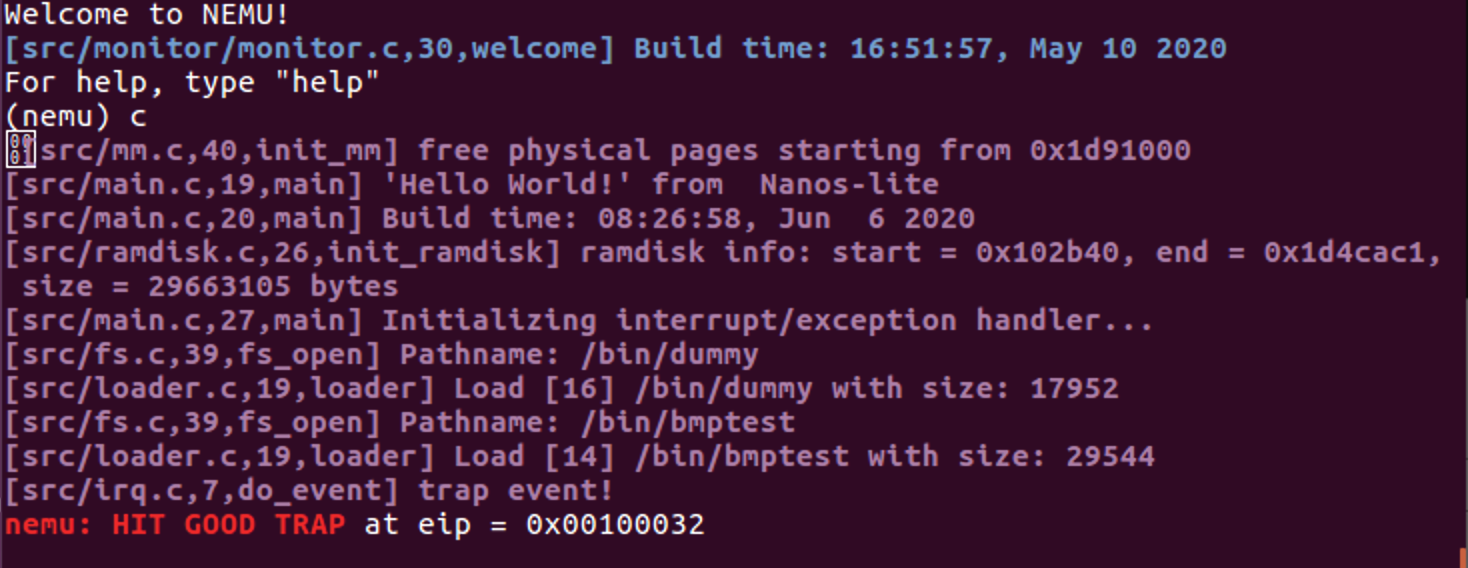
\includegraphics[scale=0.5]{fig/1.png}
    \caption{dummy加载成功}
\end{figure}
}
%——————————————————————————————————————
\subsection{分页机制上运行仙剑}
\kt{
  由于这时我们需要真正分配堆并将其映射到虚拟空间,所以前面PA3实现的一半brk需要重新进行修改使其进行真正的分配而非次次默认分配成功。首先是mm\_brk的修改使其通过\_map分配堆为[current->max\_brk, new\_brk)这一部分内存空间并将其映射到地址空间current->as中(其他部分框架代码已给出)。由于这一改动我们的堆区并不是一定可以分配成功,所以系统调用部分也要进行修改。
  \begin{lstlisting}[title=brk,frame=trbl,language={C++}]
//nanos-lite/src/mm.c
#define K4(va) (((uint32_t)(va)+0xfff) & ~0xfff)
int mm_brk(uint32_t new_brk) {
  if (current->cur_brk == 0) 
    current->cur_brk = current->max_brk = new_brk;
  else {
    if (new_brk > current->max_brk) {
      // TODO: map memory region [current->max_brk, new_brk)
      // into address space current->as
      uintptr_t va = K4(current->max_brk);
      while(va < new_brk) {
        _map(&current->as, (void *)va, (void *)new_page());
        va += PGSIZE;
      }
      current->max_brk = new_brk; 
    }
    current->cur_brk = new_brk;
  }	
  return 0;
}
//nanos-lite/src/syscall.c
case SYS_brk: SYSCALL_ARG1(r) = mm_brk(a[1]);break;//SYSCALL_ARG1(r) = 0;break;
  \end{lstlisting}
}
%---------------------------------------------------------------------------------------------------
\section{阶段二}
%——————————————————————————————————————
\subsection{上下文切换}
\kt{
  上下文切换实际上就是将当前运行程序状态(寄存器内存映射空间等)保存下来再加载另一个部分的程序状态进来,而这部分就和OS中提及的PCB相关,PCB就保存了各个进程的信息,上下文切换中的回复现场就需要用到PCB根据其内容进行恢复。
  
  所以我们需要先有一个现场才能进行上述的上下文恢复,\_umake即是如此。且由于nemu没有特权级的区别,所以在ustack的底部初始化一个以entry为返回地址的陷阱帧即可,就是构造一个有着通用寄存器以及eflags等标志位设置的陷阱帧。再之后需要同系统调用的实现一样在irq中包装事件并对其进行处理,同时还需要在trap.S中实现trap的跳转和调用。同时注释掉proc里面原来用于切换的代码改用umake初始化。

  在现场完成之后我们在进入trap陷阱中之后,需要借助调度器,即schedule函数进行上下文的切换,实际上就是指向不同的PCB交由CPU执行。
  \begin{lstlisting}[title=上下文切换,frame=trbl,language={C++}]
//nexus-am/am/arch/x86-nume/src/pte.c
_RegSet *_umake(_Protect *p, _Area ustack, _Area kstack, void *entry, char *const argv[], char *const envp[]) {
  //_umake将ustack底部初始化一个entry为返回地址的陷阱帧
  uint32_t *ptr = ustack.end;
  //navyapps程序入口函数_start的 栈帧,即8个通用寄存器
  for (int i = 0; i < 8; i++) {
	*ptr = 0x0; 
  	 ptr--;
  }
  //陷阱帧,包括栈帧的8个通用寄存器
  *ptr = 0x202; 	  
  ptr--; //eflags,即IF置1即可
  *ptr = 0x8; 	          
  ptr--; //cs 为了diff test
  *ptr = (uint32_t)entry; 
  ptr--; //eip
  *ptr = 0x0;             
  ptr--; //error code
  *ptr = 0x81;            
  ptr--; //irq id
  for (int i = 0; i < 8; i++) {
	*ptr = 0x0;
  	 ptr--;
  }
  ptr++;
  return (_RegSet *)ptr; //将会记录到tf
}
//nanos-lite/src/main.c
_trap();
//nexus-am/am/arch/x86-nemu/src/asye.c
void vectrap();
case 0x81: ev.event = _EVENT_TRAP; break;
idt[0x81] = GATE(STS_TG32, KSEL(SEG_KCODE), vectrap, DPL_USER);
//nexus-am/am/arch/x86-nemu/src/trap.S
.globl vectrap;  vectrap:  pushl $0;  pushl $0x81; jmp asm_trap
//nanos-lite/src/irq.c
case _EVENT_TRAP:return schedule(r);
//nanos-lite/src/proc.c
int count = 0;
extern int current_game;
_RegSet* schedule(_RegSet *prev) {
  //save the context pointer
  current->tf = prev;

  current =&pcb[0];
  count++;

  _switch(&current->as);
  return current->tf;
}
  \end{lstlisting}

  然后就是真的可以在虚拟内存空间——分页机制上运行仙剑了。并且同时我们的分时多任务也由于上下文切换的实现而完成了。
%——————————————————————————————————————
\subsection{分时多任务}
\kt{
  这时候基本内容都已经完成了,在proc中对schedule进行多任务切换的设定然后在main中加载多个内容即可。
    \begin{lstlisting}[title=分时多任务,frame=trbl,language={C++}]
//nanos-lite/src/proc.c
current = (current == &pcb[0] ? &pcb[1] : &pcb[0]);
//nanos-lite/src/main.c
load_prog("/bin/pal");
load_prog("/bin/hello");
    \end{lstlisting}

    可以看到如下结果在缓慢运行仙剑的时候hello也在输出,但是何必为难年幼的NEMU呢,所以后面除非必要,对仙剑的测试都只运行这一个。
  
    \begin{figure}[H]
      \centering
      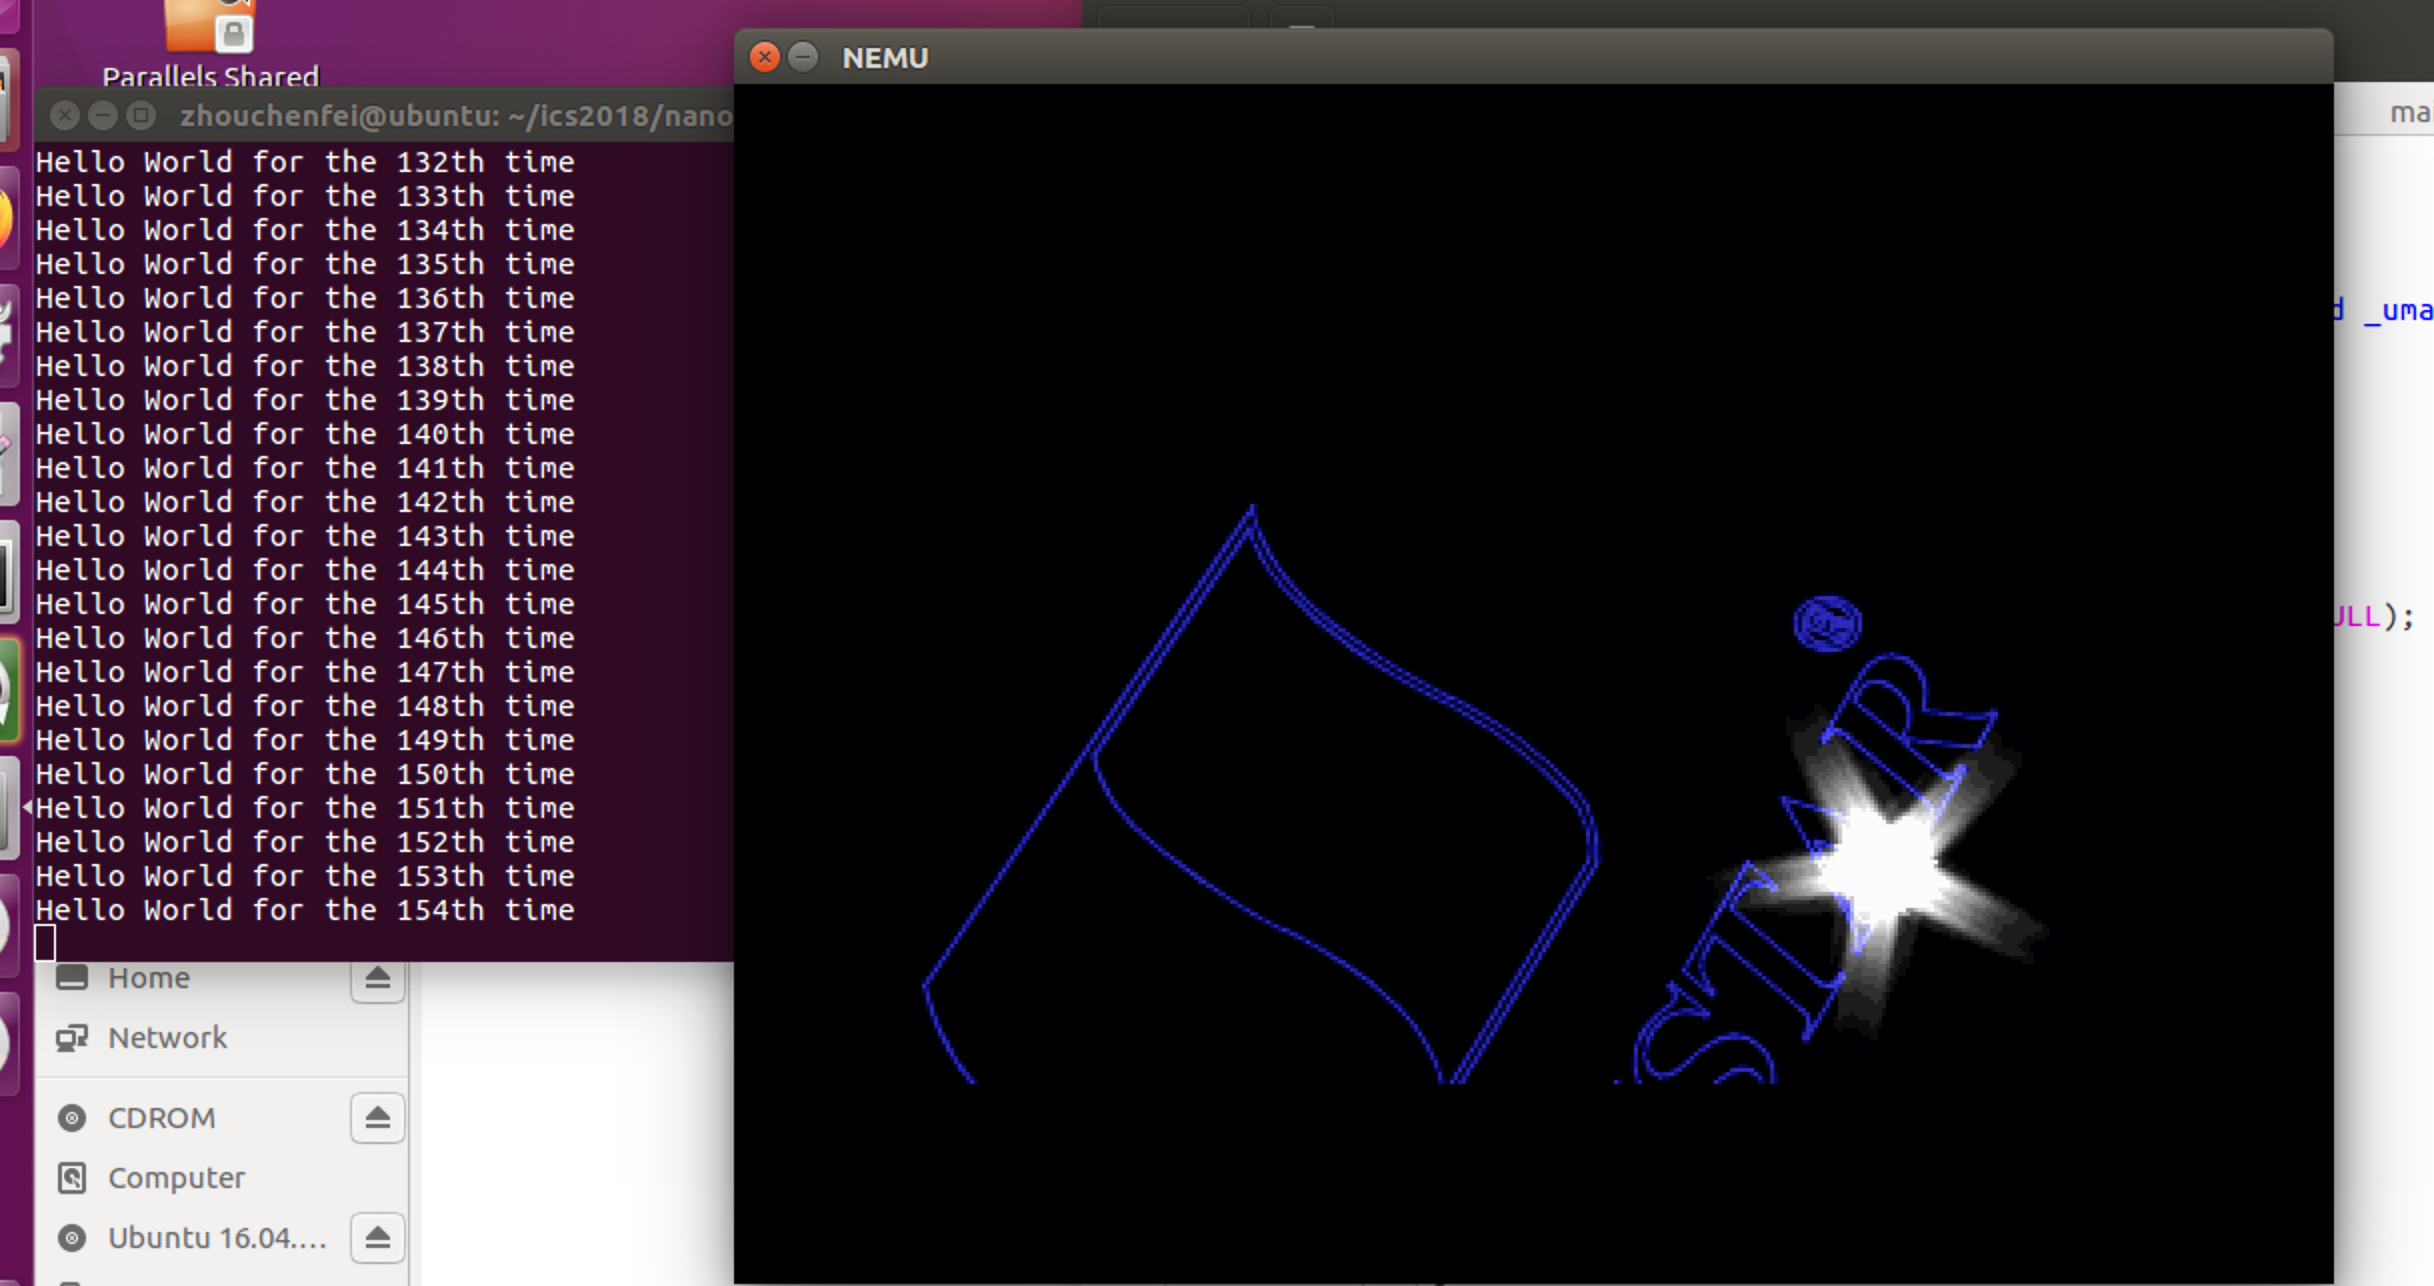
\includegraphics[scale=0.25]{fig/2.png}
      \caption{分时多任务}
  \end{figure}
}
%——————————————————————————————————————
\subsection{时间中断}
\kt{
    时间中断本质上还是中断,所以实现思路仍然与PA3的中断一致。
    \begin{lstlisting}[title=时间中断,frame=trbl,language={C++}]
//nemu/include/cpu/reg.h
//加入INTR引脚
bool INTR;
//nemu/src/cpu/intr.c
//设置为高电平
void dev_raise_intr() {
	cpu.INTR = true;
}
//nemu/src/cpu/exec/exec.c
//然后在真正的执行单元中轮询检查是否有时钟中断
#define TIMER_IRQ 0x32
  if (cpu.INTR & cpu.eflags.IF) {
	cpu.INTR = false;
	raise_intr(TIMER_IRQ, cpu.eip);
	update_eip();
  }
//同时在异常处理中对IF进行设置,使当前为关中断状态
//nemu/src/cpu/intr.c
cpu.eflags.IF = 0;
//nexus-am/am/arch/x86-nume/src/pte.c
//设置eflags
*ptr = 0x202; 	  ptr--; //eflags,即IF置1即可
//之后就是中断异常一样的处理
//nexus-am/am/arch/x86-nemu/src/asye.c
//异常号
idt[0x32] = GATE(STS_TG32, KSEL(SEG_KCODE), vectime, DPL_USER);
case 0x32: ev.event = _EVENT_IRQ_TIME; break;
//nanos-lite/src/irq.c
case _EVENT_IRQ_TIME:/*Log("_EVENT_IRQ_TIME!!");*/return schedule(r);
    \end{lstlisting}  

    如果取消Log的注释就可以看到如下结果
    \begin{figure}[H]
      \centering
      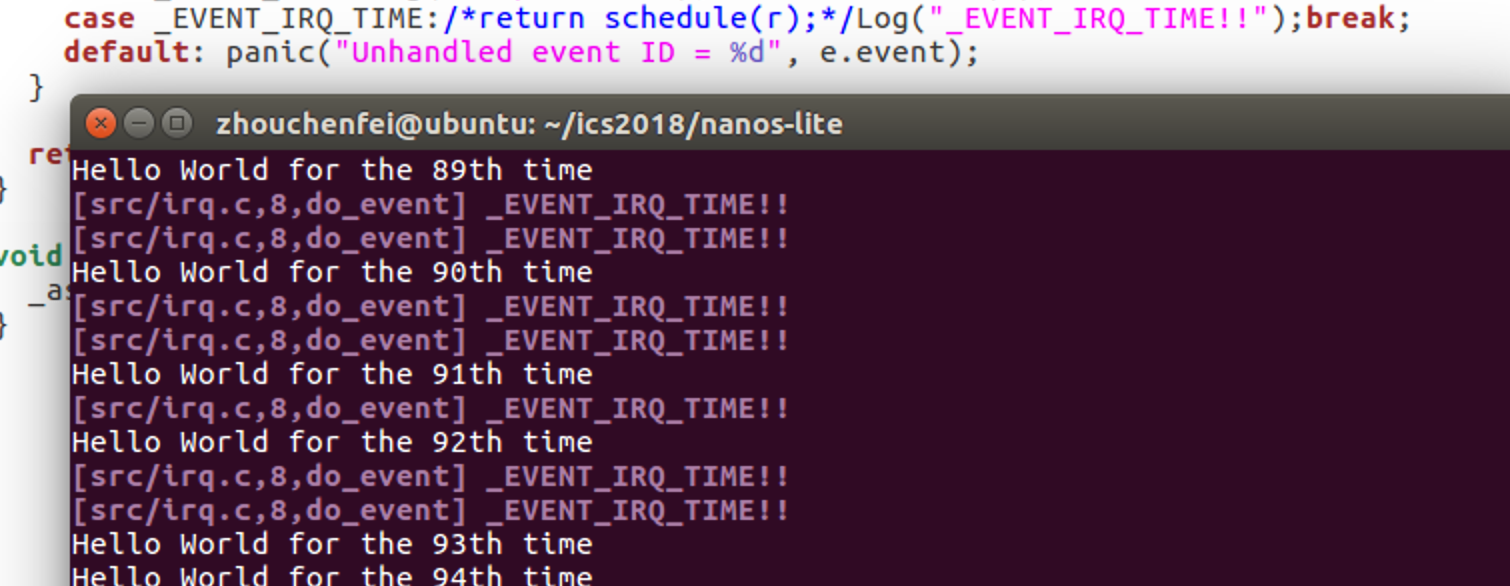
\includegraphics[scale=0.5]{fig/3.png}
      \caption{时间中断}
  \end{figure}
}
%---------------------------------------------------------------------------------------------------
\section{阶段三}
%——————————————————————————————————————
\subsection{展示系统切换}
\kt{
  首先用main加载videotest,并且在eventsread(键盘事件)中对F12按键进行识别,在F12按下的时候切换仙剑奇侠传和videotest。
  \begin{lstlisting}[title=展示,frame=trbl,language={C++}]
//nanos-lite/src/main.c
load_prog("/bin/videotest");
//nanos-lite/src/device.c
int current_game = 0;
size_t events_read(void *buf, size_t len) {
  //return 0;
	int key = _read_key();
	bool down = false;
	if (key & 0x8000) {
		key ^= 0x8000;
		down = true;
	}
	if (key == _KEY_NONE) {
		unsigned long t = _uptime();
		sprintf(buf, "t %d\n", t);
	}
	else {
		sprintf(buf, "%s %s\n", down ? "kd" : "ku", keyname[key]);
		if(key == 13 && down) { //F12 DOWN
			current_game = (current_game == 0 ? 1 : 0);
		}
		Log("Get key: %d %s %s\n", key, keyname[key], down ? "down" : "up");
	}
	return strlen(buf);
}
//nanos-lite/src/proc.c
extern int current_game;
current = (current_game == 0 ? &pcb[0] : &pcb[2]);
    \end{lstlisting}

    之后就可以成功看到切换的结果啦。

    % \begin{figure}[H]
    %     \centering
    %     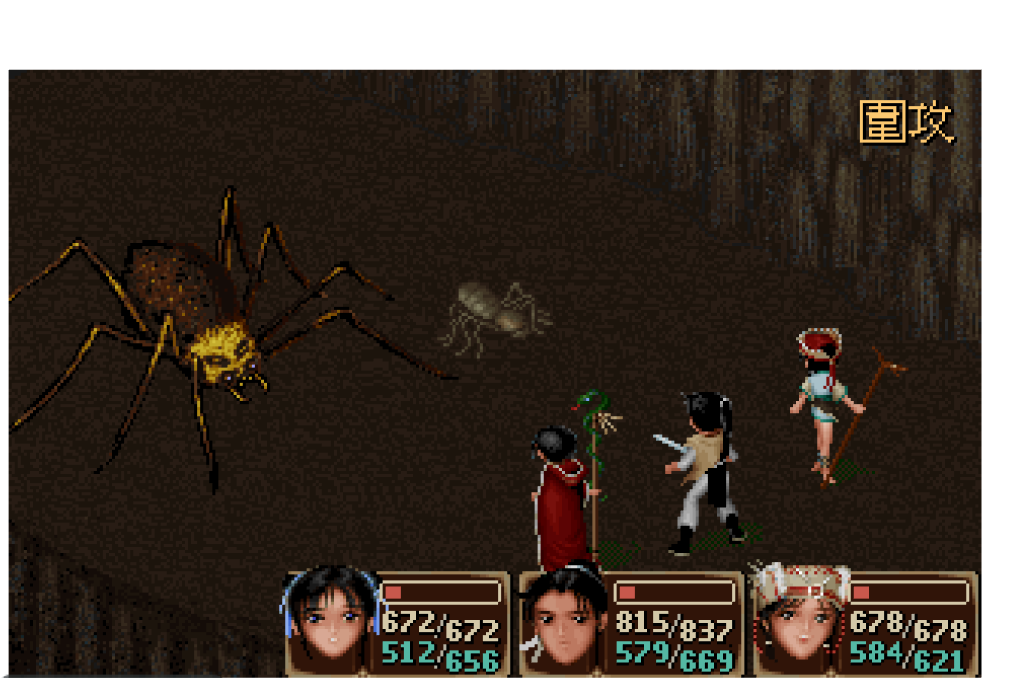
\includegraphics[scale=0.45]{fig/5.png}
    %     \caption{PASS!!}
    % \end{figure}
}
%---------------------------------------------------------------------------------------------------
\section{PA5:浮点数的支持}
\kt{
  如果不管JIT内容的话PA5简直不怎么需要时间,看懂指导书每个函数都是一句话的事情,就是仙剑运行的很慢然后存档还不好使,所以就很绝望,后来换到native上快了点,还没来得及截图,虚拟机坏了。
  \begin{lstlisting}[title=浮点数,frame=trbl,language={C++}]
//navy-apps/apps/pal/include/FLOAT.h 
static inline int F2int(FLOAT a) {
    if(a&0x80000000 == 0)
        return a/0x10000;
    else//负数
        return -((-a)/0x10000);
}

static inline FLOAT int2F(int a) {
    return a>0 ? a*0x10000: -((-a)*0x10000);
}

static inline FLOAT F_mul_int(FLOAT a, int b) {
    return a*b;
}

static inline FLOAT F_div_int(FLOAT a, int b) {
    return a/b;
}
//navy-apps/apps/pal/src/FLOAT/FLOAT.c
//解释了一大堆的部分,实际上把小数点后进行处理即可
FLOAT F_mul_F(FLOAT a, FLOAT b) {
  return a*b/0x10000;
}

FLOAT F_div_F(FLOAT a, FLOAT b) {
  return a*b*0x10000;
}
FLOAT f2F(float a) {
  /* You should figure out how to convert `a' into FLOAT without
   * introducing x87 floating point instructions. Else you can
   * not run this code in NEMU before implementing x87 floating
   * point instructions, which is contrary to our expectation.
   *
   * Hint: The bit representation of `a' is already on the
   * stack. How do you retrieve it to another variable without
   * performing arithmetic operations on it directly?
   */
  return a>0 ? a*0x10000: -((-a)*0x10000);
}

FLOAT Fabs(FLOAT a) {
  if(a&0x80000000 == 0)
    return a;
  else
    return -a;
}
  \end{lstlisting}

  然后就能战斗了。

  \begin{figure}[H]
    \centering
    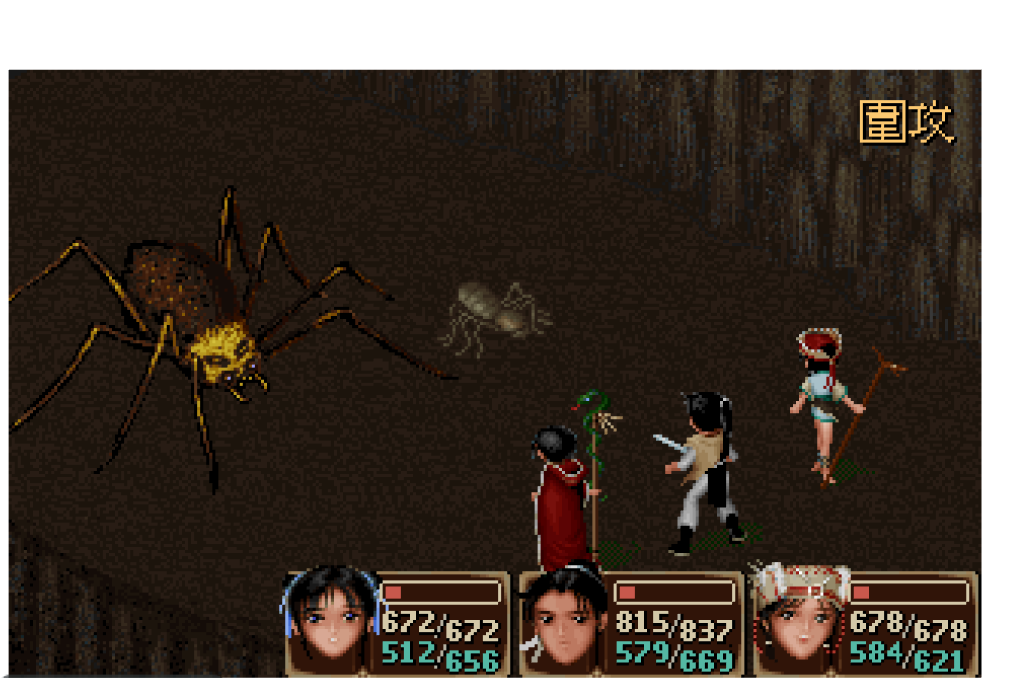
\includegraphics[scale=0.45]{fig/5.png}
    \caption{战斗}
\end{figure}

  perf的评测我本来弄了,但是虚拟机崩了没时间再弄了,就这样吧,反正也没来得及分析出什么有用的东西。
}
%---------------------------------------------------------------------------------------------------
\section{遇到的bug及解决}
\kt{
  没什么特别致命的bug,致命的是我的电脑。
    \begin{itemize}
        \item 
        \begin{todolist}
            \item [\done] 和PA3那个serial一样要先实现loader才行,我不知道是实验书真的顺序有问题还是我的理解哪里有问题
            \item [\done] PA3那个logo可以正确加载了,在实现了分页加载之后,大概就是超限了吧,不懂非要整这么个坑的意义在哪
            \item [\done] 直接make \ run切换出了一堆链接还有编译werror的错,还是clean一遍再说
            \item [\done] 时间中断作为中断也是要写在IDT表里的,80、81写好就不记得这个了
            \item [\done] 跑的再慢也不能切native,因为没法debug。。
            \item 以上问题其实还好,尚在我可以接受的范围内,但是上一次因为我不当操作导致的虚拟机崩溃我还可以忍受,这次吃个饭回来就崩的开不开机是怎么回事orz,如下图,眼看着就差个截图就可以交报告,然后什么都没了,PA3-PA5浮点数的代码还没来得及备份,完全重新来。
            
            \begin{figure}[H]
              \centering
              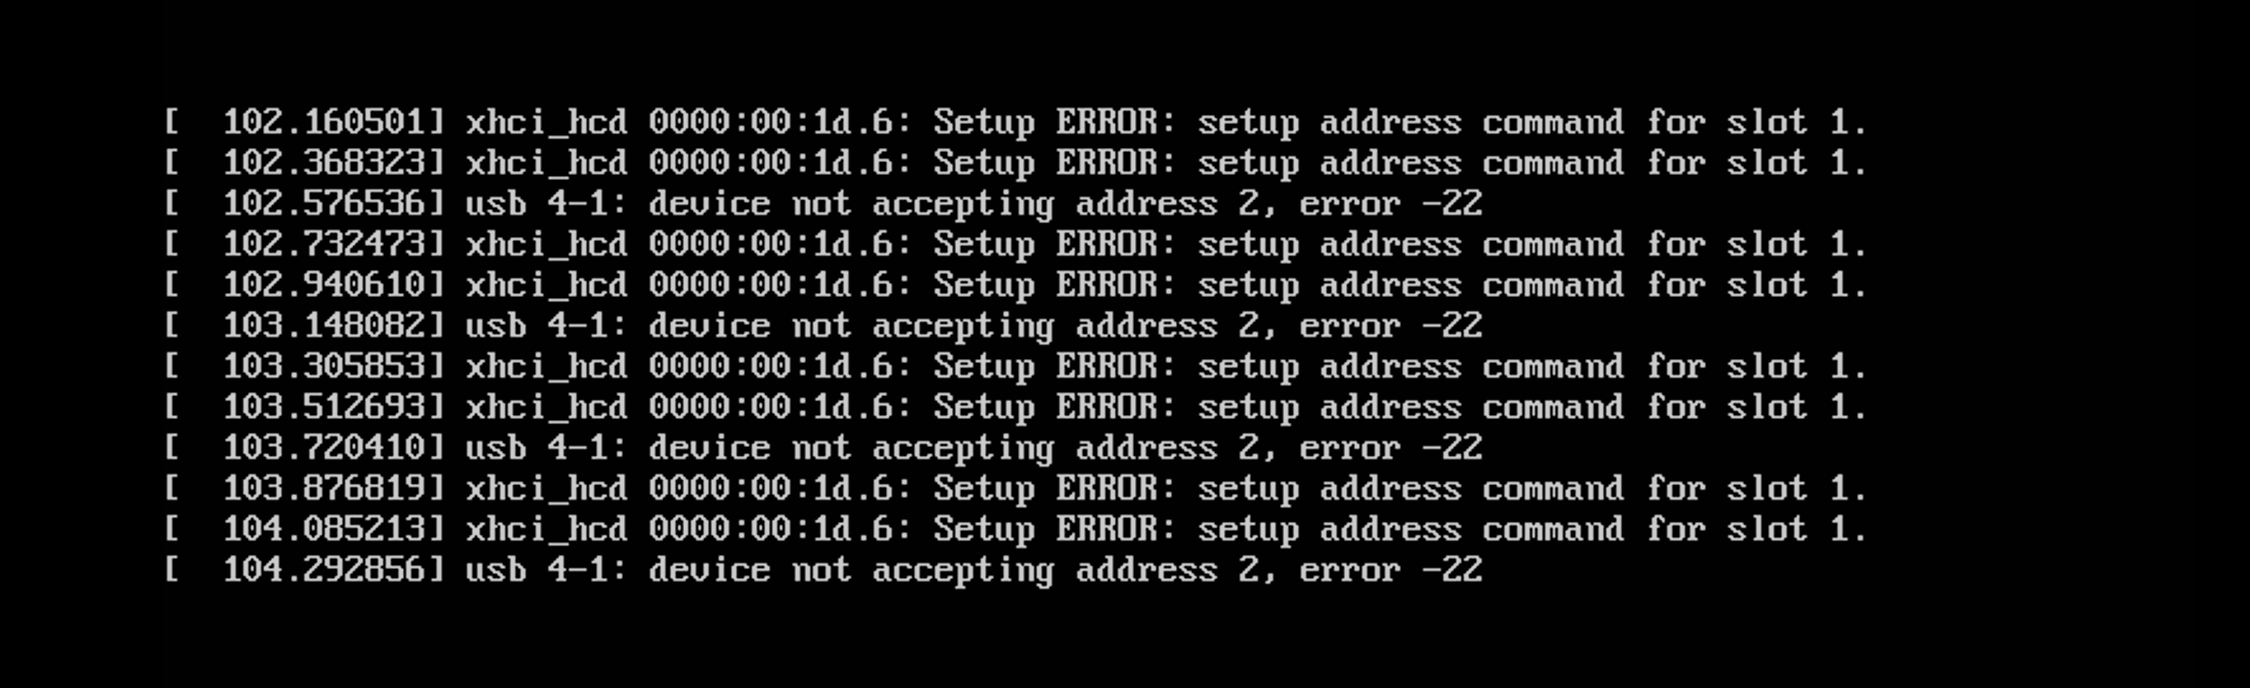
\includegraphics[scale=0.3]{fig/4.png}
              \caption{死机}
          \end{figure}
        \end{todolist}
    \end{itemize}
}
%---------------------------------------------------------------------------------------------------
\section{思考题\&\&必答题}
%——————————————————————————————————————
\subsection{思考题}
\kt{
    \begin{enumerate}
        \item 如果不同的进程共享同一个栈空间, 会发生什么呢?
        
        上下文会错乱吧。只有这部分独立才可以保证函数调用等正常执行。
        \item i386不是一个32位的处理器吗, 为什么表项中的基地址信息只有20位, 而不是32位?
        
        因为在查页目录和页表项的作用是生成20位的物理页号,最终与虚拟地址的后12位(页内地址)构成物理地址。所以这里没必要只需要使用20位基址,最后再和页内地址拼接即可,可以节省内存的开销。
        \item 手册上提到表项(包括 CR3)中的基地址都是物理地址, 物理地址是必须的吗? 能否使用虚拟地址?
        
        必须,不能使用。因为页目录和页表项均储存在内存中,到内存中寻址需要物理地址。如果表项(包括 CR3)中的基地址使用虚拟地址,那么查表得过程就要先通过MMU进行虚拟地址和物理地址得转化,这个过程中却要使用到表项,这显然是自相矛盾的。
        \item 为什么不采用一级页表? 或者说采用一级页表会有什么缺点?
        
        页表大小过大,对内存来说是一种浪费,不容易hit,或者说hit所需的时间长,开销大。
        \item 空指针真的是'空'的吗?
        
        空指针其实还是指向一个地址的,c语言中NULL的本质是(void *)0,所以空指针指向的是0这个地址,而这个地址不与其他实际地址冲突
    \end{enumerate}
}
%——————————————————————————————————————
\subsection{必答题}
\kt{
    以下以外的必答题均为代码实现。
    \begin{enumerate}
        \item 分时多任务的具体过程 请结合代码, 解释分页机制和硬件中断是如何支撑仙剑奇侠传和hello程序在我们的计算机系统(Nanos-lite, AM, NEMU)中分时运行的.
        
        时间中断每到一定时间触发一次,然后引起硬件中断yield,中断前会保存上下文,然后yield会使用schedule进行调度,调度器选择下一个将要被执行的程序,如仙剑切到hello,选择之后根据pcb的内容对该pcb的上下文进行载入恢复,然后cpu继续执行,如此往复。

    \end{enumerate}
}
%----------------------------------------------------------------------------- 
\section{总结}
\kt{
    
    没有什么好总结的,没写报告前写完PA5浮点数的时候是非常开心的,因为很早就完成了任务,然后开始写报告并且又一次运行看看有没有bug的时候虚拟机崩掉的时候就只想赶紧弄好赶紧扔掉完事,虽然确实成长了许多,也确实找到了许多丢三落四自己作死导致的天坑,但是远没有吃个饭电脑充着电虚拟机就突然黑屏再也打不开来的坑大,因为这次机制特殊用的虚拟机所以没有很好的把代码同github同步,然后因为想着可能还有问题就不去备份代码调好了再备份,然后就多花了不知道多少时间恢复代码,是不是和以前一样有没有更多的bug也没有精力去管了。所幸前面的截图还能找到记录,报告不用被耽误,且由于pa4开始变为2018但代码保留的是2019的就很头疼,所以想借jyb同学的docker镜像一用(省去环境配置时间),结果Mac的ssh又开始抽风。本想着等代码彻底复原了再提交报告,现在看来是没有什么可能了,毕竟照着写好的报告粘都能粘出问题。祝贺PA完结,大三下死亡生活结束。

    终于隔了两天算是把代码复原了吧,最终版本用的最简单古早的2018代码,实在不想折腾各种乱七八糟的东西了,Mac上Xquartz连不上,用vmware在2019的显示上又有一点小问题。所以最后用的Mac上的虚拟机ParallelDesktop安装了ubuntu系统并运行nemu代码。发现了即使流程大致记得代码完全粘贴复现也还是会暴露不少问题,还有一些前面忽视的细节的小坑。一言蔽之,对指导书的理解还需加深。
    }
%----------------------------------------------------------------------------- 
% \lhead{\kaishu 参考文献}
% \newpage
% \kt{
% \begin{thebibliography}{plain}  
%     \bibitem{ref1}Ray Tracing经典入门[EB/OL].https://raytracing.github.io/books/
%     \bibitem{ref2}讲稿lec2-5,8
% \end{thebibliography}
% }
\end{document}
